\documentclass[twoside]{book}

% Packages required by doxygen
\usepackage{fixltx2e}
\usepackage{calc}
\usepackage{doxygen}
\usepackage[export]{adjustbox} % also loads graphicx
\usepackage{graphicx}
\usepackage[utf8]{inputenc}
\usepackage{makeidx}
\usepackage{multicol}
\usepackage{multirow}
\PassOptionsToPackage{warn}{textcomp}
\usepackage{textcomp}
\usepackage[nointegrals]{wasysym}
\usepackage[table]{xcolor}

% Font selection
\usepackage[T1]{fontenc}
\usepackage[scaled=.90]{helvet}
\usepackage{courier}
\usepackage{amssymb}
\usepackage{sectsty}
\renewcommand{\familydefault}{\sfdefault}
\allsectionsfont{%
  \fontseries{bc}\selectfont%
  \color{darkgray}%
}
\renewcommand{\DoxyLabelFont}{%
  \fontseries{bc}\selectfont%
  \color{darkgray}%
}
\newcommand{\+}{\discretionary{\mbox{\scriptsize$\hookleftarrow$}}{}{}}

% Page & text layout
\usepackage{geometry}
\geometry{%
  a4paper,%
  top=2.5cm,%
  bottom=2.5cm,%
  left=2.5cm,%
  right=2.5cm%
}
\tolerance=750
\hfuzz=15pt
\hbadness=750
\setlength{\emergencystretch}{15pt}
\setlength{\parindent}{0cm}
\setlength{\parskip}{3ex plus 2ex minus 2ex}
\makeatletter
\renewcommand{\paragraph}{%
  \@startsection{paragraph}{4}{0ex}{-1.0ex}{1.0ex}{%
    \normalfont\normalsize\bfseries\SS@parafont%
  }%
}
\renewcommand{\subparagraph}{%
  \@startsection{subparagraph}{5}{0ex}{-1.0ex}{1.0ex}{%
    \normalfont\normalsize\bfseries\SS@subparafont%
  }%
}
\makeatother

% Headers & footers
\usepackage{fancyhdr}
\pagestyle{fancyplain}
\fancyhead[LE]{\fancyplain{}{\bfseries\thepage}}
\fancyhead[CE]{\fancyplain{}{}}
\fancyhead[RE]{\fancyplain{}{\bfseries\leftmark}}
\fancyhead[LO]{\fancyplain{}{\bfseries\rightmark}}
\fancyhead[CO]{\fancyplain{}{}}
\fancyhead[RO]{\fancyplain{}{\bfseries\thepage}}
\fancyfoot[LE]{\fancyplain{}{}}
\fancyfoot[CE]{\fancyplain{}{}}
\fancyfoot[RE]{\fancyplain{}{\bfseries\scriptsize Generated by Doxygen }}
\fancyfoot[LO]{\fancyplain{}{\bfseries\scriptsize Generated by Doxygen }}
\fancyfoot[CO]{\fancyplain{}{}}
\fancyfoot[RO]{\fancyplain{}{}}
\renewcommand{\footrulewidth}{0.4pt}
\renewcommand{\chaptermark}[1]{%
  \markboth{#1}{}%
}
\renewcommand{\sectionmark}[1]{%
  \markright{\thesection\ #1}%
}

% Indices & bibliography
\usepackage{natbib}
\usepackage[titles]{tocloft}
\setcounter{tocdepth}{3}
\setcounter{secnumdepth}{5}
\makeindex

% Hyperlinks (required, but should be loaded last)
\usepackage{ifpdf}
\ifpdf
  \usepackage[pdftex,pagebackref=true]{hyperref}
\else
  \usepackage[ps2pdf,pagebackref=true]{hyperref}
\fi
\hypersetup{%
  colorlinks=true,%
  linkcolor=blue,%
  citecolor=blue,%
  unicode%
}

% Custom commands
\newcommand{\clearemptydoublepage}{%
  \newpage{\pagestyle{empty}\cleardoublepage}%
}

\usepackage{caption}
\captionsetup{labelsep=space,justification=centering,font={bf},singlelinecheck=off,skip=4pt,position=top}

%===== C O N T E N T S =====

\begin{document}

% Titlepage & ToC
\hypersetup{pageanchor=false,
             bookmarksnumbered=true,
             pdfencoding=unicode
            }
\pagenumbering{alph}
\begin{titlepage}
\vspace*{7cm}
\begin{center}%
{\Large Arbutus\+Engine }\\
\vspace*{1cm}
{\large Generated by Doxygen 1.8.13}\\
\end{center}
\end{titlepage}
\clearemptydoublepage
\pagenumbering{roman}
\tableofcontents
\clearemptydoublepage
\pagenumbering{arabic}
\hypersetup{pageanchor=true}

%--- Begin generated contents ---
\chapter{Hierarchical Index}
\section{Class Hierarchy}
This inheritance list is sorted roughly, but not completely, alphabetically\+:\begin{DoxyCompactList}
\item \contentsline{section}{Engine}{\pageref{class_engine}}{}
\item of\+Thread\begin{DoxyCompactList}
\item \contentsline{section}{File\+Manager}{\pageref{class_file_manager}}{}
\end{DoxyCompactList}
\end{DoxyCompactList}

\chapter{Class Index}
\section{Class List}
Here are the classes, structs, unions and interfaces with brief descriptions\+:\begin{DoxyCompactList}
\item\contentsline{section}{\hyperlink{class_engine}{Engine} \\*The main class, used to control all aspects of the Arbutus V\+Jing Library }{\pageref{class_engine}}{}
\item\contentsline{section}{\hyperlink{class_file_manager}{File\+Manager} }{\pageref{class_file_manager}}{}
\end{DoxyCompactList}

\chapter{Class Documentation}
\hypertarget{class_engine}{}\section{Engine Class Reference}
\label{class_engine}\index{Engine@{Engine}}


The main class, used to control all aspects of the Arbutus V\+Jing Library.  




{\ttfamily \#include $<$Engine.\+h$>$}

\subsection*{Public Member Functions}
\begin{DoxyCompactItemize}
\item 
void \hyperlink{class_engine_a7b198cae741a0031f89dab6844e44ed2}{setup\+Syphon} ()
\item 
bool \hyperlink{class_engine_adc03481dd61714c7bfc3ffe48e2772a9}{new\+Set} (unsigned int \+\_\+width=0, unsigned int \+\_\+height=0, unsigned int \+\_\+layers=0)
\item 
void \hyperlink{class_engine_a360e63d1c939cc8a70f0cd2fd289fc87}{close\+Set} ()
\item 
bool \hyperlink{class_engine_ae1aab6389f4cc21cf760689f95c6d298}{open\+Set} (string \+\_\+set\+Path)
\item 
bool \hyperlink{class_engine_abdf0e7642de80e72a9a64c559d2af9ba}{save\+Set} ()
\item 
bool \hyperlink{class_engine_a699dad06243f1f462f9e2f6f6e33cbdb}{save\+Set\+As} (string \+\_\+set\+Path)
\item 
void \hyperlink{class_engine_a368d1d6924b49241c994b2857606421b}{set\+Mixer\+Resolution} (unsigned int width, unsigned int height)
\item 
void \hyperlink{class_engine_a5633281e514055b66fde30596305d646}{handle\+Layer\+Action} (string parameter, json data)
\item 
void \hyperlink{class_engine_a8342ba4b8e00754a5dc78e9590df4fbb}{handle\+Visual\+Action} (string parameter, json data)
\item 
void \hyperlink{class_engine_ae25acfdee442242b7c1262f02f8b7274}{handle\+Action} (string parameter, json data)
\item 
void \hyperlink{class_engine_a7ad20895ed6034844683fd2190bbd911}{play} (json data)
\item 
void \hyperlink{class_engine_a1c64956ca2429493e66c8aa0e5f3d23f}{stop} (json data)
\item 
Visual\+Instance $\ast$ \hyperlink{class_engine_a8527a1c21e96b85c113efac943f83039}{set\+Active\+Visual\+Instance} (unsigned int layerN, unsigned int columnN)
\item 
void \hyperlink{class_engine_a9f4d3c2ac126aa622fa464300d1d361c}{set\+Active\+Visual\+Intances} (unsigned int columnN)
\item 
void \hyperlink{class_engine_a4800f622ab7b7125d70aea8c0426dbb3}{set\+Active\+Visual\+Intance\+On\+Active\+Layer} (unsigned int visual\+InstanceN)
\item 
Visual\+Instance $\ast$ \hyperlink{class_engine_a0cd50c81fc1479d3afa3b847151fa086}{get\+Current\+Active\+Visual\+Instance} ()
\item 
Visual\+Instance $\ast$ \hyperlink{class_engine_acd81098a646a2918353c66a9bb86f63e}{get\+Visual\+At\+Layer\+And\+InstanceN} (unsigned int layerN, unsigned int visual\+InstanceN)
\item 
Layer\+Properties $\ast$ \hyperlink{class_engine_af1868ab55619c4eceb1dce26bd7a0182}{get\+Properties\+Of\+Current\+Layer} ()
\item 
Scene $\ast$ \hyperlink{class_engine_a4e9d4666046294e3d2ce91b21ce67571}{add\+Scene} ()
\item 
void \hyperlink{class_engine_a6e9b7c17e564a3f10c9cb7301d64ecb4}{add\+Visual\+To\+Scene\+List\+In\+Current\+Layer} (unsigned int visual, unsigned int layer, unsigned int column)
\item 
void \hyperlink{class_engine_afc245ab31c528fe807f45309772de07b}{add\+Visual\+To\+Scene} (unsigned int visual, unsigned int layer, unsigned int column)
\item 
void \hyperlink{class_engine_af8b450a6e2bb5979b4216a143e010045}{remove\+Visual\+From\+Scene} (unsigned int layer, unsigned int column)
\item 
Scene $\ast$ \hyperlink{class_engine_ab81eff238bf568d470ba149e51be0c45}{get\+Current\+Scene} ()
\item 
Scene $\ast$ \hyperlink{class_engine_a161746a86c8a635a1552f6184a9381e6}{get\+Scene\+At\+Index} (unsigned int index)
\item 
unsigned int \hyperlink{class_engine_a02161314b59b98413587878fbe74bda0}{get\+Number\+Of\+Visuals} ()
\item 
Visual $\ast$ \hyperlink{class_engine_a3104acd7a59d71021bc513e6a48b6536}{get\+Visual\+At\+Index} (unsigned int index)
\item 
bool \hyperlink{class_engine_a3c973c85ef1912fc5d50c582ddb2d135}{is\+Syphon\+Input\+Loaded} (string server\+Name, string app\+Name)
\item 
Visual\+Syphon $\ast$ \hyperlink{class_engine_acd0e841800f3376e2629298d9225a72b}{get\+Syphon\+Input} (string server\+Name, string app\+Name)
\item 
json \hyperlink{class_engine_aafca00518b99bb4c493d3206d5c3bf9f}{get\+State} ()
\item 
void \hyperlink{class_engine_aa04b3d433a32a2b7baa6df9141d7a911}{set\+State} (json state)
\item 
json \hyperlink{class_engine_ae66a8b01a9d58d880b744de54e0ac431}{get\+Layers\+State} ()
\item 
\mbox{\Hypertarget{class_engine_a7960743aefd62e846e7f3cd92c18bc73}\label{class_engine_a7960743aefd62e846e7f3cd92c18bc73}} 
void {\bfseries render} ()
\item 
\mbox{\Hypertarget{class_engine_a564b2faadbe929f38aa02cdd4436ece6}\label{class_engine_a564b2faadbe929f38aa02cdd4436ece6}} 
void {\bfseries draw\+Output} (int x=0, int y=0, int width=0, int height=0)
\item 
\mbox{\Hypertarget{class_engine_a565a7f269e754b894d91bf76070b4cdd}\label{class_engine_a565a7f269e754b894d91bf76070b4cdd}} 
void {\bfseries draw\+Layer} (int layer\+Number, int x, int y, int width, int height)
\item 
\mbox{\Hypertarget{class_engine_a7f7a7d140a8bba36827d6f7086528ac5}\label{class_engine_a7f7a7d140a8bba36827d6f7086528ac5}} 
void {\bfseries draw\+Output\+Preview} (int x, int y, int width, int height)
\item 
\mbox{\Hypertarget{class_engine_ab17e462ac3798478f26a96ad92125c4e}\label{class_engine_ab17e462ac3798478f26a96ad92125c4e}} 
void {\bfseries draw\+Layers\+Preview} (int x, int y, int height, int max\+Num\+Layers=M\+A\+X\+I\+M\+U\+M\+\_\+\+N\+U\+M\+B\+E\+R\+\_\+\+O\+F\+\_\+\+L\+A\+Y\+E\+RS)
\item 
\mbox{\Hypertarget{class_engine_aaf8e3940d24161c0f997b72d589068b8}\label{class_engine_aaf8e3940d24161c0f997b72d589068b8}} 
void {\bfseries print\+Info} ()
\item 
\mbox{\Hypertarget{class_engine_a664e672344fe4b517afd8a69032f15d0}\label{class_engine_a664e672344fe4b517afd8a69032f15d0}} 
void {\bfseries save\+Current\+Frame} (string path)
\item 
\mbox{\Hypertarget{class_engine_abbe2df9eae88e6533ee3359c298c0b0d}\label{class_engine_abbe2df9eae88e6533ee3359c298c0b0d}} 
void {\bfseries beat} ()
\item 
\mbox{\Hypertarget{class_engine_ad34cbad27b16111b2ac1918ad94ee040}\label{class_engine_ad34cbad27b16111b2ac1918ad94ee040}} 
void {\bfseries start\+Metronome} ()
\item 
\mbox{\Hypertarget{class_engine_a15599493b7802e76e5c9d41c809780c4}\label{class_engine_a15599493b7802e76e5c9d41c809780c4}} 
void {\bfseries stop\+Metronome} ()
\item 
\mbox{\Hypertarget{class_engine_ab65eac2d82aa0d8111e9a4b2e6d0ecc1}\label{class_engine_ab65eac2d82aa0d8111e9a4b2e6d0ecc1}} 
void {\bfseries tap} ()
\item 
\mbox{\Hypertarget{class_engine_a353f4e05ddda3cc59c8f1771f71662c6}\label{class_engine_a353f4e05ddda3cc59c8f1771f71662c6}} 
void {\bfseries set\+B\+PM} (unsigned int new\+B\+PM)
\item 
\mbox{\Hypertarget{class_engine_a047a41c1296190a69107b4aac41ccaed}\label{class_engine_a047a41c1296190a69107b4aac41ccaed}} 
unsigned int {\bfseries get\+B\+PM} ()
\item 
\mbox{\Hypertarget{class_engine_a7047f8df5a9c5607dbb61dbec043b3f0}\label{class_engine_a7047f8df5a9c5607dbb61dbec043b3f0}} 
void {\bfseries trigger\+Schedulled\+Visuals\+On\+All\+Layers} ()
\item 
\mbox{\Hypertarget{class_engine_aa087714d3b0cc57d7ef830307eec34d7}\label{class_engine_aa087714d3b0cc57d7ef830307eec34d7}} 
void {\bfseries reset\+Metronome} ()
\item 
\mbox{\Hypertarget{class_engine_a499ded081fc30ca383551920dfbe2da9}\label{class_engine_a499ded081fc30ca383551920dfbe2da9}} 
unsigned int {\bfseries get\+Current\+Beat} ()
\item 
\mbox{\Hypertarget{class_engine_a4de047df829801ba27022c4ae69d7722}\label{class_engine_a4de047df829801ba27022c4ae69d7722}} 
void {\bfseries init\+Buffer} ()
\item 
\mbox{\Hypertarget{class_engine_a824d9fdae22ed6832f8c353880bdc6c4}\label{class_engine_a824d9fdae22ed6832f8c353880bdc6c4}} 
void {\bfseries destroy\+Buffer} ()
\item 
\mbox{\Hypertarget{class_engine_a5f19d013ac5499d1b1a3f4ebd2169964}\label{class_engine_a5f19d013ac5499d1b1a3f4ebd2169964}} 
void {\bfseries key\+Pressed} (int key)
\item 
\mbox{\Hypertarget{class_engine_a2d598300be2dc442672e3f8bf3d30c5a}\label{class_engine_a2d598300be2dc442672e3f8bf3d30c5a}} 
void {\bfseries key\+Released} (int key)
\item 
\mbox{\Hypertarget{class_engine_ae4b6b116aa4d6c5890fda96e83f4ae20}\label{class_engine_ae4b6b116aa4d6c5890fda96e83f4ae20}} 
void {\bfseries mouse\+Moved} (int x, int y)
\item 
\mbox{\Hypertarget{class_engine_a428c8e164c2f0f01b07d8179ff6e21e0}\label{class_engine_a428c8e164c2f0f01b07d8179ff6e21e0}} 
void {\bfseries mouse\+Dragged} (int x, int y, int button)
\item 
\mbox{\Hypertarget{class_engine_a7ce4ba1856c33c19ee104fcd6bb47633}\label{class_engine_a7ce4ba1856c33c19ee104fcd6bb47633}} 
void {\bfseries mouse\+Pressed} (int x, int y, int button)
\item 
\mbox{\Hypertarget{class_engine_a5f8775f5a9fa94f608bce7b07a4e711a}\label{class_engine_a5f8775f5a9fa94f608bce7b07a4e711a}} 
void {\bfseries mouse\+Released} (int x, int y, int button)
\item 
\mbox{\Hypertarget{class_engine_a276e8d0c9e083bc5adab1ccade6b6674}\label{class_engine_a276e8d0c9e083bc5adab1ccade6b6674}} 
void {\bfseries set\+Defaults} ()
\item 
\mbox{\Hypertarget{class_engine_a0116b74bb312164086fe9ee3e5fd9d5b}\label{class_engine_a0116b74bb312164086fe9ee3e5fd9d5b}} 
void {\bfseries scan\+Cameras} ()
\item 
\mbox{\Hypertarget{class_engine_a18dcb065818c6ec7e76168452eb45001}\label{class_engine_a18dcb065818c6ec7e76168452eb45001}} 
void {\bfseries cleanup} ()
\item 
\mbox{\Hypertarget{class_engine_a9e7f54a907c2e058295edba5a59ef578}\label{class_engine_a9e7f54a907c2e058295edba5a59ef578}} 
void {\bfseries change\+Midi\+Port} (int port)
\item 
\mbox{\Hypertarget{class_engine_ab5e53de6ca336844026f6cf4858abd77}\label{class_engine_ab5e53de6ca336844026f6cf4858abd77}} 
void {\bfseries change\+Osc\+Port} (int port)
\item 
\mbox{\Hypertarget{class_engine_add90fd5f0eb935ef688127c741baa35e}\label{class_engine_add90fd5f0eb935ef688127c741baa35e}} 
string {\bfseries get\+Current\+File\+Path} ()
\item 
\mbox{\Hypertarget{class_engine_a69aa9d5f07000a38eaaeae6c5f33f800}\label{class_engine_a69aa9d5f07000a38eaaeae6c5f33f800}} 
of\+Fbo $\ast$ {\bfseries get\+Buffer} ()
\item 
\mbox{\Hypertarget{class_engine_a1fbd799ded9ac4b7a27f57ff0364468e}\label{class_engine_a1fbd799ded9ac4b7a27f57ff0364468e}} 
void {\bfseries set\+App\+Support\+Dir} (string \+\_\+dir)
\item 
\mbox{\Hypertarget{class_engine_a5307012b50388efb4e359540e328c468}\label{class_engine_a5307012b50388efb4e359540e328c468}} 
string {\bfseries calculate\+Thumbnail\+Path} (string path)
\item 
void \hyperlink{class_engine_a3cf7820fd1dc335f82218ec6a9ef355b}{register\+App\+Beat\+Callback} (void($\ast$callback)(void))
\end{DoxyCompactItemize}
\subsection*{Static Public Member Functions}
\begin{DoxyCompactItemize}
\item 
static \hyperlink{class_engine}{Engine} $\ast$ \hyperlink{class_engine_ae8f7319cf3683c23f6a215952d47ebdf}{get\+Instance} ()
\item 
\mbox{\Hypertarget{class_engine_a74e15b996e9dcc8c89c3d1e3e944f07d}\label{class_engine_a74e15b996e9dcc8c89c3d1e3e944f07d}} 
static void {\bfseries visuals\+Keys\+Control\+Callback} (Controller $\ast$controller)
\end{DoxyCompactItemize}
\subsection*{Public Attributes}
\begin{DoxyCompactItemize}
\item 
\mbox{\Hypertarget{class_engine_a3cd1207cb568ad1f8628c3d1720175b6}\label{class_engine_a3cd1207cb568ad1f8628c3d1720175b6}} 
dispatch\+\_\+queue\+\_\+t {\bfseries processing\+Queue}
\item 
\mbox{\Hypertarget{class_engine_a5d74ea26de11bd68eb1c94a2580508a6}\label{class_engine_a5d74ea26de11bd68eb1c94a2580508a6}} 
void($\ast$ {\bfseries app\+Beat\+Callback} )(void)
\end{DoxyCompactItemize}


\subsection{Detailed Description}
The main class, used to control all aspects of the Arbutus V\+Jing Library. 

This class implements the singleton pattƒ\+Layerern to create one object used to manage all aspects of the Arbutus \hyperlink{class_engine}{Engine}. 

\subsection{Member Function Documentation}
\mbox{\Hypertarget{class_engine_a4e9d4666046294e3d2ce91b21ce67571}\label{class_engine_a4e9d4666046294e3d2ce91b21ce67571}} 
\index{Engine@{Engine}!add\+Scene@{add\+Scene}}
\index{add\+Scene@{add\+Scene}!Engine@{Engine}}
\subsubsection{\texorpdfstring{add\+Scene()}{addScene()}}
{\footnotesize\ttfamily Scene $\ast$ Engine\+::add\+Scene (\begin{DoxyParamCaption}{ }\end{DoxyParamCaption})}

... \mbox{\Hypertarget{class_engine_afc245ab31c528fe807f45309772de07b}\label{class_engine_afc245ab31c528fe807f45309772de07b}} 
\index{Engine@{Engine}!add\+Visual\+To\+Scene@{add\+Visual\+To\+Scene}}
\index{add\+Visual\+To\+Scene@{add\+Visual\+To\+Scene}!Engine@{Engine}}
\subsubsection{\texorpdfstring{add\+Visual\+To\+Scene()}{addVisualToScene()}}
{\footnotesize\ttfamily void Engine\+::add\+Visual\+To\+Scene (\begin{DoxyParamCaption}\item[{unsigned int}]{visual,  }\item[{unsigned int}]{layer,  }\item[{unsigned int}]{column }\end{DoxyParamCaption})}

... \mbox{\Hypertarget{class_engine_a6e9b7c17e564a3f10c9cb7301d64ecb4}\label{class_engine_a6e9b7c17e564a3f10c9cb7301d64ecb4}} 
\index{Engine@{Engine}!add\+Visual\+To\+Scene\+List\+In\+Current\+Layer@{add\+Visual\+To\+Scene\+List\+In\+Current\+Layer}}
\index{add\+Visual\+To\+Scene\+List\+In\+Current\+Layer@{add\+Visual\+To\+Scene\+List\+In\+Current\+Layer}!Engine@{Engine}}
\subsubsection{\texorpdfstring{add\+Visual\+To\+Scene\+List\+In\+Current\+Layer()}{addVisualToSceneListInCurrentLayer()}}
{\footnotesize\ttfamily void Engine\+::add\+Visual\+To\+Scene\+List\+In\+Current\+Layer (\begin{DoxyParamCaption}\item[{unsigned int}]{visual,  }\item[{unsigned int}]{layer,  }\item[{unsigned int}]{column }\end{DoxyParamCaption})}

... \mbox{\Hypertarget{class_engine_a360e63d1c939cc8a70f0cd2fd289fc87}\label{class_engine_a360e63d1c939cc8a70f0cd2fd289fc87}} 
\index{Engine@{Engine}!close\+Set@{close\+Set}}
\index{close\+Set@{close\+Set}!Engine@{Engine}}
\subsubsection{\texorpdfstring{close\+Set()}{closeSet()}}
{\footnotesize\ttfamily void Engine\+::close\+Set (\begin{DoxyParamCaption}{ }\end{DoxyParamCaption})}

Closes a set and cleans up the memory \mbox{\Hypertarget{class_engine_a0cd50c81fc1479d3afa3b847151fa086}\label{class_engine_a0cd50c81fc1479d3afa3b847151fa086}} 
\index{Engine@{Engine}!get\+Current\+Active\+Visual\+Instance@{get\+Current\+Active\+Visual\+Instance}}
\index{get\+Current\+Active\+Visual\+Instance@{get\+Current\+Active\+Visual\+Instance}!Engine@{Engine}}
\subsubsection{\texorpdfstring{get\+Current\+Active\+Visual\+Instance()}{getCurrentActiveVisualInstance()}}
{\footnotesize\ttfamily Visual\+Instance $\ast$ Engine\+::get\+Current\+Active\+Visual\+Instance (\begin{DoxyParamCaption}{ }\end{DoxyParamCaption})}

... \mbox{\Hypertarget{class_engine_ab81eff238bf568d470ba149e51be0c45}\label{class_engine_ab81eff238bf568d470ba149e51be0c45}} 
\index{Engine@{Engine}!get\+Current\+Scene@{get\+Current\+Scene}}
\index{get\+Current\+Scene@{get\+Current\+Scene}!Engine@{Engine}}
\subsubsection{\texorpdfstring{get\+Current\+Scene()}{getCurrentScene()}}
{\footnotesize\ttfamily Scene $\ast$ Engine\+::get\+Current\+Scene (\begin{DoxyParamCaption}{ }\end{DoxyParamCaption})}

... \mbox{\Hypertarget{class_engine_ae8f7319cf3683c23f6a215952d47ebdf}\label{class_engine_ae8f7319cf3683c23f6a215952d47ebdf}} 
\index{Engine@{Engine}!get\+Instance@{get\+Instance}}
\index{get\+Instance@{get\+Instance}!Engine@{Engine}}
\subsubsection{\texorpdfstring{get\+Instance()}{getInstance()}}
{\footnotesize\ttfamily \hyperlink{class_engine}{Engine} $\ast$ Engine\+::get\+Instance (\begin{DoxyParamCaption}{ }\end{DoxyParamCaption})\hspace{0.3cm}{\ttfamily [static]}}

Singleton instance getter \mbox{\Hypertarget{class_engine_ae66a8b01a9d58d880b744de54e0ac431}\label{class_engine_ae66a8b01a9d58d880b744de54e0ac431}} 
\index{Engine@{Engine}!get\+Layers\+State@{get\+Layers\+State}}
\index{get\+Layers\+State@{get\+Layers\+State}!Engine@{Engine}}
\subsubsection{\texorpdfstring{get\+Layers\+State()}{getLayersState()}}
{\footnotesize\ttfamily json Engine\+::get\+Layers\+State (\begin{DoxyParamCaption}{ }\end{DoxyParamCaption})}

... \mbox{\Hypertarget{class_engine_a02161314b59b98413587878fbe74bda0}\label{class_engine_a02161314b59b98413587878fbe74bda0}} 
\index{Engine@{Engine}!get\+Number\+Of\+Visuals@{get\+Number\+Of\+Visuals}}
\index{get\+Number\+Of\+Visuals@{get\+Number\+Of\+Visuals}!Engine@{Engine}}
\subsubsection{\texorpdfstring{get\+Number\+Of\+Visuals()}{getNumberOfVisuals()}}
{\footnotesize\ttfamily unsigned int Engine\+::get\+Number\+Of\+Visuals (\begin{DoxyParamCaption}{ }\end{DoxyParamCaption})}

... \mbox{\Hypertarget{class_engine_af1868ab55619c4eceb1dce26bd7a0182}\label{class_engine_af1868ab55619c4eceb1dce26bd7a0182}} 
\index{Engine@{Engine}!get\+Properties\+Of\+Current\+Layer@{get\+Properties\+Of\+Current\+Layer}}
\index{get\+Properties\+Of\+Current\+Layer@{get\+Properties\+Of\+Current\+Layer}!Engine@{Engine}}
\subsubsection{\texorpdfstring{get\+Properties\+Of\+Current\+Layer()}{getPropertiesOfCurrentLayer()}}
{\footnotesize\ttfamily Layer\+Properties$\ast$ Engine\+::get\+Properties\+Of\+Current\+Layer (\begin{DoxyParamCaption}{ }\end{DoxyParamCaption})}

... \mbox{\Hypertarget{class_engine_a161746a86c8a635a1552f6184a9381e6}\label{class_engine_a161746a86c8a635a1552f6184a9381e6}} 
\index{Engine@{Engine}!get\+Scene\+At\+Index@{get\+Scene\+At\+Index}}
\index{get\+Scene\+At\+Index@{get\+Scene\+At\+Index}!Engine@{Engine}}
\subsubsection{\texorpdfstring{get\+Scene\+At\+Index()}{getSceneAtIndex()}}
{\footnotesize\ttfamily Scene $\ast$ Engine\+::get\+Scene\+At\+Index (\begin{DoxyParamCaption}\item[{unsigned int}]{index }\end{DoxyParamCaption})}

... \mbox{\Hypertarget{class_engine_aafca00518b99bb4c493d3206d5c3bf9f}\label{class_engine_aafca00518b99bb4c493d3206d5c3bf9f}} 
\index{Engine@{Engine}!get\+State@{get\+State}}
\index{get\+State@{get\+State}!Engine@{Engine}}
\subsubsection{\texorpdfstring{get\+State()}{getState()}}
{\footnotesize\ttfamily json Engine\+::get\+State (\begin{DoxyParamCaption}{ }\end{DoxyParamCaption})}

... \mbox{\Hypertarget{class_engine_acd0e841800f3376e2629298d9225a72b}\label{class_engine_acd0e841800f3376e2629298d9225a72b}} 
\index{Engine@{Engine}!get\+Syphon\+Input@{get\+Syphon\+Input}}
\index{get\+Syphon\+Input@{get\+Syphon\+Input}!Engine@{Engine}}
\subsubsection{\texorpdfstring{get\+Syphon\+Input()}{getSyphonInput()}}
{\footnotesize\ttfamily Visual\+Syphon $\ast$ Engine\+::get\+Syphon\+Input (\begin{DoxyParamCaption}\item[{string}]{server\+Name,  }\item[{string}]{app\+Name }\end{DoxyParamCaption})}

... \mbox{\Hypertarget{class_engine_a3104acd7a59d71021bc513e6a48b6536}\label{class_engine_a3104acd7a59d71021bc513e6a48b6536}} 
\index{Engine@{Engine}!get\+Visual\+At\+Index@{get\+Visual\+At\+Index}}
\index{get\+Visual\+At\+Index@{get\+Visual\+At\+Index}!Engine@{Engine}}
\subsubsection{\texorpdfstring{get\+Visual\+At\+Index()}{getVisualAtIndex()}}
{\footnotesize\ttfamily Visual $\ast$ Engine\+::get\+Visual\+At\+Index (\begin{DoxyParamCaption}\item[{unsigned int}]{index }\end{DoxyParamCaption})}

... \mbox{\Hypertarget{class_engine_acd81098a646a2918353c66a9bb86f63e}\label{class_engine_acd81098a646a2918353c66a9bb86f63e}} 
\index{Engine@{Engine}!get\+Visual\+At\+Layer\+And\+InstanceN@{get\+Visual\+At\+Layer\+And\+InstanceN}}
\index{get\+Visual\+At\+Layer\+And\+InstanceN@{get\+Visual\+At\+Layer\+And\+InstanceN}!Engine@{Engine}}
\subsubsection{\texorpdfstring{get\+Visual\+At\+Layer\+And\+Instance\+N()}{getVisualAtLayerAndInstanceN()}}
{\footnotesize\ttfamily Visual\+Instance $\ast$ Engine\+::get\+Visual\+At\+Layer\+And\+InstanceN (\begin{DoxyParamCaption}\item[{unsigned int}]{layerN,  }\item[{unsigned int}]{visual\+InstanceN }\end{DoxyParamCaption})}

... \mbox{\Hypertarget{class_engine_ae25acfdee442242b7c1262f02f8b7274}\label{class_engine_ae25acfdee442242b7c1262f02f8b7274}} 
\index{Engine@{Engine}!handle\+Action@{handle\+Action}}
\index{handle\+Action@{handle\+Action}!Engine@{Engine}}
\subsubsection{\texorpdfstring{handle\+Action()}{handleAction()}}
{\footnotesize\ttfamily void Engine\+::handle\+Action (\begin{DoxyParamCaption}\item[{string}]{parameter,  }\item[{json}]{data }\end{DoxyParamCaption})}

handles all actions to the engine 
\begin{DoxyParams}{Parameters}
{\em parameter} & a string \\
\hline
\end{DoxyParams}
\mbox{\Hypertarget{class_engine_a5633281e514055b66fde30596305d646}\label{class_engine_a5633281e514055b66fde30596305d646}} 
\index{Engine@{Engine}!handle\+Layer\+Action@{handle\+Layer\+Action}}
\index{handle\+Layer\+Action@{handle\+Layer\+Action}!Engine@{Engine}}
\subsubsection{\texorpdfstring{handle\+Layer\+Action()}{handleLayerAction()}}
{\footnotesize\ttfamily void Engine\+::handle\+Layer\+Action (\begin{DoxyParamCaption}\item[{string}]{parameter,  }\item[{json}]{data }\end{DoxyParamCaption})}

handles all actions related to layers \mbox{\Hypertarget{class_engine_a8342ba4b8e00754a5dc78e9590df4fbb}\label{class_engine_a8342ba4b8e00754a5dc78e9590df4fbb}} 
\index{Engine@{Engine}!handle\+Visual\+Action@{handle\+Visual\+Action}}
\index{handle\+Visual\+Action@{handle\+Visual\+Action}!Engine@{Engine}}
\subsubsection{\texorpdfstring{handle\+Visual\+Action()}{handleVisualAction()}}
{\footnotesize\ttfamily void Engine\+::handle\+Visual\+Action (\begin{DoxyParamCaption}\item[{string}]{parameter,  }\item[{json}]{data }\end{DoxyParamCaption})}

handles all actions related to visuals \mbox{\Hypertarget{class_engine_a3c973c85ef1912fc5d50c582ddb2d135}\label{class_engine_a3c973c85ef1912fc5d50c582ddb2d135}} 
\index{Engine@{Engine}!is\+Syphon\+Input\+Loaded@{is\+Syphon\+Input\+Loaded}}
\index{is\+Syphon\+Input\+Loaded@{is\+Syphon\+Input\+Loaded}!Engine@{Engine}}
\subsubsection{\texorpdfstring{is\+Syphon\+Input\+Loaded()}{isSyphonInputLoaded()}}
{\footnotesize\ttfamily bool Engine\+::is\+Syphon\+Input\+Loaded (\begin{DoxyParamCaption}\item[{string}]{server\+Name,  }\item[{string}]{app\+Name }\end{DoxyParamCaption})}

...

Traverse all the inputs, check if they are syphon inputs, check if the servername and appname are the samse \mbox{\Hypertarget{class_engine_adc03481dd61714c7bfc3ffe48e2772a9}\label{class_engine_adc03481dd61714c7bfc3ffe48e2772a9}} 
\index{Engine@{Engine}!new\+Set@{new\+Set}}
\index{new\+Set@{new\+Set}!Engine@{Engine}}
\subsubsection{\texorpdfstring{new\+Set()}{newSet()}}
{\footnotesize\ttfamily bool Engine\+::new\+Set (\begin{DoxyParamCaption}\item[{unsigned int}]{\+\_\+width = {\ttfamily 0},  }\item[{unsigned int}]{\+\_\+height = {\ttfamily 0},  }\item[{unsigned int}]{\+\_\+layers = {\ttfamily 0} }\end{DoxyParamCaption})}

Starts a new set with the given dimentions and number of layers. Also allocs all memory needed. 
\begin{DoxyParams}{Parameters}
{\em \+\_\+width} & the width of the rendering area \\
\hline
{\em \+\_\+height} & the height of the rendering area \\
\hline
{\em \+\_\+layers} & the number of layers available \\
\hline
\end{DoxyParams}
\begin{DoxyReturn}{Returns}
a boolean result saying if the set was properly created or not 
\end{DoxyReturn}
\mbox{\Hypertarget{class_engine_ae1aab6389f4cc21cf760689f95c6d298}\label{class_engine_ae1aab6389f4cc21cf760689f95c6d298}} 
\index{Engine@{Engine}!open\+Set@{open\+Set}}
\index{open\+Set@{open\+Set}!Engine@{Engine}}
\subsubsection{\texorpdfstring{open\+Set()}{openSet()}}
{\footnotesize\ttfamily bool Engine\+::open\+Set (\begin{DoxyParamCaption}\item[{string}]{\+\_\+set\+Path }\end{DoxyParamCaption})}

Open a set 
\begin{DoxyParams}{Parameters}
{\em \+\_\+set\+Path} & the path to the file to open \\
\hline
\end{DoxyParams}
\begin{DoxyReturn}{Returns}
open success value. boolean 
\end{DoxyReturn}
\mbox{\Hypertarget{class_engine_a7ad20895ed6034844683fd2190bbd911}\label{class_engine_a7ad20895ed6034844683fd2190bbd911}} 
\index{Engine@{Engine}!play@{play}}
\index{play@{play}!Engine@{Engine}}
\subsubsection{\texorpdfstring{play()}{play()}}
{\footnotesize\ttfamily void Engine\+::play (\begin{DoxyParamCaption}\item[{json}]{data }\end{DoxyParamCaption})}

... \mbox{\Hypertarget{class_engine_a3cf7820fd1dc335f82218ec6a9ef355b}\label{class_engine_a3cf7820fd1dc335f82218ec6a9ef355b}} 
\index{Engine@{Engine}!register\+App\+Beat\+Callback@{register\+App\+Beat\+Callback}}
\index{register\+App\+Beat\+Callback@{register\+App\+Beat\+Callback}!Engine@{Engine}}
\subsubsection{\texorpdfstring{register\+App\+Beat\+Callback()}{registerAppBeatCallback()}}
{\footnotesize\ttfamily void Engine\+::register\+App\+Beat\+Callback (\begin{DoxyParamCaption}\item[{void($\ast$)(void)}]{callback }\end{DoxyParamCaption})}

Register the callback to be executed on the app when a beat occurs 
\begin{DoxyParams}{Parameters}
{\em void$\ast$} & callback the callback to be executed \\
\hline
\end{DoxyParams}
\mbox{\Hypertarget{class_engine_af8b450a6e2bb5979b4216a143e010045}\label{class_engine_af8b450a6e2bb5979b4216a143e010045}} 
\index{Engine@{Engine}!remove\+Visual\+From\+Scene@{remove\+Visual\+From\+Scene}}
\index{remove\+Visual\+From\+Scene@{remove\+Visual\+From\+Scene}!Engine@{Engine}}
\subsubsection{\texorpdfstring{remove\+Visual\+From\+Scene()}{removeVisualFromScene()}}
{\footnotesize\ttfamily void Engine\+::remove\+Visual\+From\+Scene (\begin{DoxyParamCaption}\item[{unsigned int}]{layer,  }\item[{unsigned int}]{column }\end{DoxyParamCaption})}

... \mbox{\Hypertarget{class_engine_abdf0e7642de80e72a9a64c559d2af9ba}\label{class_engine_abdf0e7642de80e72a9a64c559d2af9ba}} 
\index{Engine@{Engine}!save\+Set@{save\+Set}}
\index{save\+Set@{save\+Set}!Engine@{Engine}}
\subsubsection{\texorpdfstring{save\+Set()}{saveSet()}}
{\footnotesize\ttfamily bool Engine\+::save\+Set (\begin{DoxyParamCaption}{ }\end{DoxyParamCaption})}

Saves the set to the current filepath \begin{DoxyReturn}{Returns}
boolean the result 
\end{DoxyReturn}
\mbox{\Hypertarget{class_engine_a699dad06243f1f462f9e2f6f6e33cbdb}\label{class_engine_a699dad06243f1f462f9e2f6f6e33cbdb}} 
\index{Engine@{Engine}!save\+Set\+As@{save\+Set\+As}}
\index{save\+Set\+As@{save\+Set\+As}!Engine@{Engine}}
\subsubsection{\texorpdfstring{save\+Set\+As()}{saveSetAs()}}
{\footnotesize\ttfamily bool Engine\+::save\+Set\+As (\begin{DoxyParamCaption}\item[{string}]{\+\_\+set\+Path }\end{DoxyParamCaption})}

Saves a VJ set into a file 
\begin{DoxyParams}{Parameters}
{\em \+\_\+set\+Path} & the path to the file to save \\
\hline
\end{DoxyParams}
\begin{DoxyReturn}{Returns}
a boolean result. True if the file as saved and false if not 
\end{DoxyReturn}
\mbox{\Hypertarget{class_engine_a8527a1c21e96b85c113efac943f83039}\label{class_engine_a8527a1c21e96b85c113efac943f83039}} 
\index{Engine@{Engine}!set\+Active\+Visual\+Instance@{set\+Active\+Visual\+Instance}}
\index{set\+Active\+Visual\+Instance@{set\+Active\+Visual\+Instance}!Engine@{Engine}}
\subsubsection{\texorpdfstring{set\+Active\+Visual\+Instance()}{setActiveVisualInstance()}}
{\footnotesize\ttfamily Visual\+Instance $\ast$ Engine\+::set\+Active\+Visual\+Instance (\begin{DoxyParamCaption}\item[{unsigned int}]{layerN,  }\item[{unsigned int}]{columnN }\end{DoxyParamCaption})}

... W\+H\+AT IS A\+LL T\+H\+IS???? W\+H\+AT IS IT D\+O\+I\+NG. sending the one really playing? \mbox{\Hypertarget{class_engine_a4800f622ab7b7125d70aea8c0426dbb3}\label{class_engine_a4800f622ab7b7125d70aea8c0426dbb3}} 
\index{Engine@{Engine}!set\+Active\+Visual\+Intance\+On\+Active\+Layer@{set\+Active\+Visual\+Intance\+On\+Active\+Layer}}
\index{set\+Active\+Visual\+Intance\+On\+Active\+Layer@{set\+Active\+Visual\+Intance\+On\+Active\+Layer}!Engine@{Engine}}
\subsubsection{\texorpdfstring{set\+Active\+Visual\+Intance\+On\+Active\+Layer()}{setActiveVisualIntanceOnActiveLayer()}}
{\footnotesize\ttfamily void Engine\+::set\+Active\+Visual\+Intance\+On\+Active\+Layer (\begin{DoxyParamCaption}\item[{unsigned int}]{visual\+InstanceN }\end{DoxyParamCaption})}

... \mbox{\Hypertarget{class_engine_a9f4d3c2ac126aa622fa464300d1d361c}\label{class_engine_a9f4d3c2ac126aa622fa464300d1d361c}} 
\index{Engine@{Engine}!set\+Active\+Visual\+Intances@{set\+Active\+Visual\+Intances}}
\index{set\+Active\+Visual\+Intances@{set\+Active\+Visual\+Intances}!Engine@{Engine}}
\subsubsection{\texorpdfstring{set\+Active\+Visual\+Intances()}{setActiveVisualIntances()}}
{\footnotesize\ttfamily void Engine\+::set\+Active\+Visual\+Intances (\begin{DoxyParamCaption}\item[{unsigned int}]{columnN }\end{DoxyParamCaption})}

... \mbox{\Hypertarget{class_engine_a368d1d6924b49241c994b2857606421b}\label{class_engine_a368d1d6924b49241c994b2857606421b}} 
\index{Engine@{Engine}!set\+Mixer\+Resolution@{set\+Mixer\+Resolution}}
\index{set\+Mixer\+Resolution@{set\+Mixer\+Resolution}!Engine@{Engine}}
\subsubsection{\texorpdfstring{set\+Mixer\+Resolution()}{setMixerResolution()}}
{\footnotesize\ttfamily void Engine\+::set\+Mixer\+Resolution (\begin{DoxyParamCaption}\item[{unsigned int}]{width,  }\item[{unsigned int}]{height }\end{DoxyParamCaption})}

Defines the area of the rendering buffer \mbox{\Hypertarget{class_engine_aa04b3d433a32a2b7baa6df9141d7a911}\label{class_engine_aa04b3d433a32a2b7baa6df9141d7a911}} 
\index{Engine@{Engine}!set\+State@{set\+State}}
\index{set\+State@{set\+State}!Engine@{Engine}}
\subsubsection{\texorpdfstring{set\+State()}{setState()}}
{\footnotesize\ttfamily void Engine\+::set\+State (\begin{DoxyParamCaption}\item[{json}]{state }\end{DoxyParamCaption})}

... \mbox{\Hypertarget{class_engine_a7b198cae741a0031f89dab6844e44ed2}\label{class_engine_a7b198cae741a0031f89dab6844e44ed2}} 
\index{Engine@{Engine}!setup\+Syphon@{setup\+Syphon}}
\index{setup\+Syphon@{setup\+Syphon}!Engine@{Engine}}
\subsubsection{\texorpdfstring{setup\+Syphon()}{setupSyphon()}}
{\footnotesize\ttfamily void Engine\+::setup\+Syphon (\begin{DoxyParamCaption}{ }\end{DoxyParamCaption})}

setup some syphon outputs this is temporary. needs to be controlled by the user and stored on the file \mbox{\Hypertarget{class_engine_a1c64956ca2429493e66c8aa0e5f3d23f}\label{class_engine_a1c64956ca2429493e66c8aa0e5f3d23f}} 
\index{Engine@{Engine}!stop@{stop}}
\index{stop@{stop}!Engine@{Engine}}
\subsubsection{\texorpdfstring{stop()}{stop()}}
{\footnotesize\ttfamily void Engine\+::stop (\begin{DoxyParamCaption}\item[{json}]{data }\end{DoxyParamCaption})}

... 

The documentation for this class was generated from the following files\+:\begin{DoxyCompactItemize}
\item 
src/\+Library/\+Engine/Engine.\+h\item 
src/\+Library/\+Engine/Engine.\+mm\end{DoxyCompactItemize}

\hypertarget{class_file_manager}{}\section{File\+Manager Class Reference}
\label{class_file_manager}\index{File\+Manager@{File\+Manager}}
Inheritance diagram for File\+Manager\+:\begin{figure}[H]
\begin{center}
\leavevmode
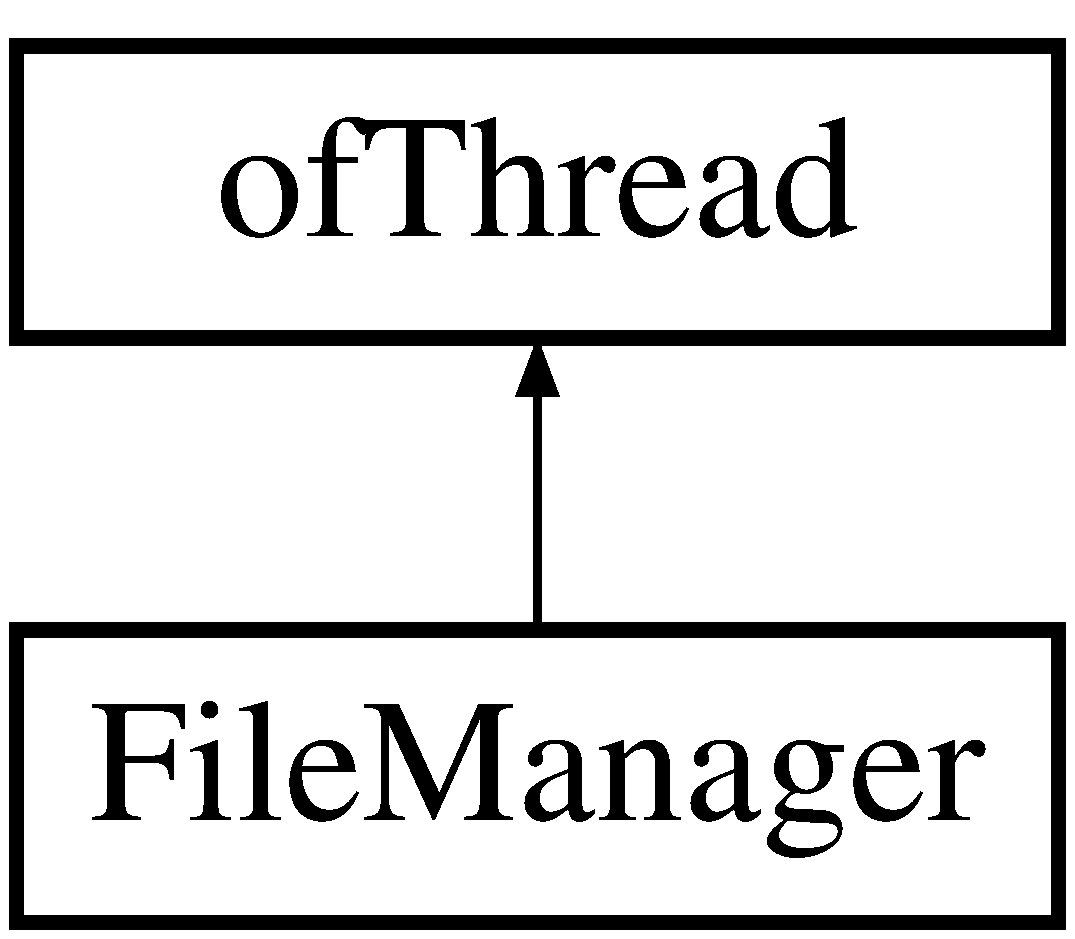
\includegraphics[height=2.000000cm]{class_file_manager}
\end{center}
\end{figure}
\subsection*{Public Member Functions}
\begin{DoxyCompactItemize}
\item 
\mbox{\Hypertarget{class_file_manager_a62d032b875c7f4d9fd8dd63366c84ac4}\label{class_file_manager_a62d032b875c7f4d9fd8dd63366c84ac4}} 
void {\bfseries start} ()
\item 
\mbox{\Hypertarget{class_file_manager_acaab8093e052afae216f8436af2f283e}\label{class_file_manager_acaab8093e052afae216f8436af2f283e}} 
void {\bfseries stop} ()
\item 
\mbox{\Hypertarget{class_file_manager_a96ba4b1661fc67fcb71de944002c1ce5}\label{class_file_manager_a96ba4b1661fc67fcb71de944002c1ce5}} 
void {\bfseries reset} ()
\item 
\mbox{\Hypertarget{class_file_manager_aee35ffdb32676b67f49f133cf0155b04}\label{class_file_manager_aee35ffdb32676b67f49f133cf0155b04}} 
void {\bfseries threaded\+Function} ()
\end{DoxyCompactItemize}


The documentation for this class was generated from the following files\+:\begin{DoxyCompactItemize}
\item 
src/\+Library/\+Engine/File\+Manager.\+h\item 
src/\+Library/\+Engine/File\+Manager.\+mm\end{DoxyCompactItemize}

%--- End generated contents ---

% Index
\backmatter
\newpage
\phantomsection
\clearemptydoublepage
\addcontentsline{toc}{chapter}{Index}
\printindex

\end{document}
